% !TeX root = ../FoodSpy.tex
% \section{Tehnologii}

\section{MikroORM și ORM}
ORM sau Object-Relational Mapping este o tehnică de a interoga și manipula datele dintr-o bază de date folosind o paradigmă orientată pe obiect. MikroORM este o bibliotecă TypeScript care implementează această tehnică.
MikroORM încapsulează codul necesar manevrării datelor și astfel nu mai este nevoie de scrierea explicită a interogărilor.
\\ \\
Mai mult, biblioteca permite interacțiunea directă cu obiectele din baza de date folosind același limbaj în care este scris codul-sursă al aplicației - în cazul nostru, TypeScript.
\\ \\
MikroORM prezintă o serie de avantaje printre care faptul că utilizarea procedurilor stocate sau a tranzacțiilor se face la fel de simplu precum un apel de funcție, dar și faptul că modelul de date este definit o singură dată, ceea ce îl face ușor de actualizat și menținut. Un exemplu de model de date este ”User”. ”User” modelează utilizatorul aplicației, prin câmpuri precum ”email”, și este reprezentat în (Fig. \ref{fig:51}).

\begin{figure}[!htb]
	\centering
	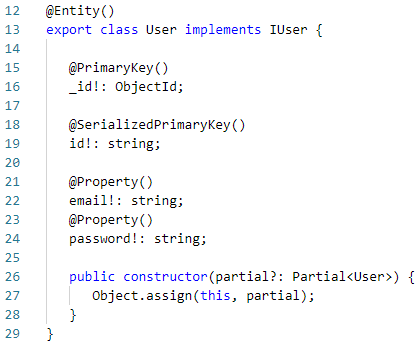
\includegraphics
	{../LaTeX/Images/mikroorm_user.PNG}
	\caption{Model de date MikroORM}
	\label{fig:51}
\end{figure}


\section{MongoDB și MongoDB Atlas}
MongoDB este un sistem de gestiune a bazelor de date orientat pe document. Deoarece un document este asemenea unui obiect JSON, câmpurile conținute în acesta pot să difere de la document la document și de asemenea, structura acestuia se poate modifica de-a lungul timpului. MongoDB permite o asociere directă între documentul din baza de date și obiectul din codul-sursă al aplicației, oferind programatorului posibilitatea de a manipula datele cu ușurință.

\begin{figure}[!htb]
	\centering
	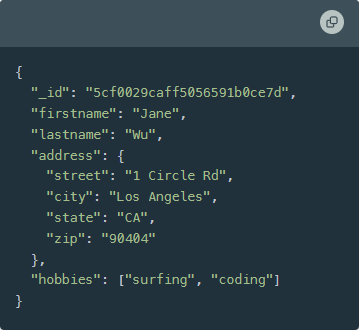
\includegraphics
	{../LaTeX/Images/mongodb_document.PNG}
	\caption{Document MongoDB}
	\label{fig:52}
\end{figure}

%maybe add \\ \\ here
La rădăcini, MongoDB este un sistem de gestiune scalabil și pretabil pentru a rula pe sisteme distribuite - aici intervine MongoDB Atlas care este serviciul MongoDB găzduit în cloud. Atlas pune la dispoziție toate funcționalitățile serviciului MongoDB, dar în același timp automatizează partea de administrare a bazei de date, de la configurarea acesteia până la efectuarea operației de ”backup”.
\\ \\
În oferta de găzduire în cloud există și un nivel gratis, așa numitul ”M0 Sandbox”, care poate fi folosit pentru acomodare cu serviciul MongoDB, pentru prototipare și pentru primele implementări ale bazei de date.


\section{Node.js}
Node.js este un mediu de rulare JavaScript construit pe engine-ul V8 din Chrome. Este folosit pentru a rula aplicații web în afara browser-ului clientului. Deoarece folosește un mediu de rulare asincron, bazat pe evenimente, Node.js este gândit pentru scalabilitatea aplicațiilor de rețea, fiind capabil să administreze un număr mare de conexiuni în mod concurent.
\\ \\
Un modul Node.js este asemenea unei librării JavaScript care poate fi inclus înăuntrul unei aplicații pentru a facilita anumite funcționalități. De exemplu, în (Fig. \ref{fig:53}) este ilustrată utilizarea modului HTTP care face posibil crearea unui server web, care ascultă pe portul 2000.

\begin{figure}[!htb]
	\centering
	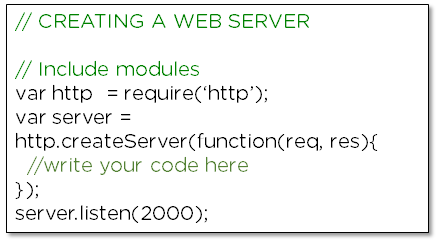
\includegraphics[width=0.8\textwidth]
	{../LaTeX/Images/nodejs_http.PNG}
	\caption{Modulul HTTP din Node.js}
	\label{fig:53}
\end{figure}

Față de mediul de rulare convențional, bazat pe thread-uri, Node.js are avantajul că funcțiile nu execută operații de input / output, deci procesul de rulare al aplicației nu este blocat niciodată. Mai mult, librăria Express din Node.js poate fi utilizată în diferite scenarii, de la aplicații de chat în timp real până la API-uri REST.


\section{Express}
Node.js nu oferă suport pentru diferitele verbe HTTP, precum GET, POST sau DELETE. De asemenea, nu poate servi fișiere statice și nici nu poate trata cererile care pot veni la diferite URL-uri, așa numitele ”rute” sau ”endpoint”-uri. Pentru aceste cazuri, este necesară implementarea manuală sau folosirea unui framework web, în speță, Express.
\\ \\
Express adresează neajunsurile Node.js enumerate mai sus prin pachete ”middleware” și, mai mult decât atât, aceste pachete pot fi folosite pentru lucrul cu sesiuni sau cookie-uri, extragerea parametrilor din URL sau a datelor transmise prin corpul cererilor POST.

\begin{figure}[!htb]
	\centering
	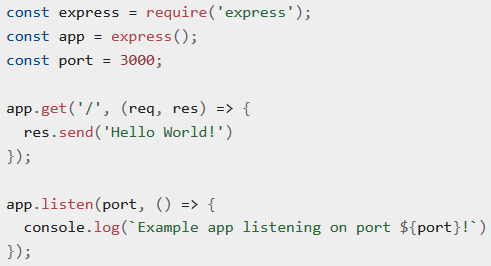
\includegraphics
	{../LaTeX/Images/express_hello.PNG}
	\caption{”Hello World” în Express}
	\label{fig:54}
\end{figure}

%maybe add \\ \\ here
Inițial, se importă modulul Express prin ”require(‘express’)”. Aplicația Express se instanțiază prin ”const app = express()”. Cu ajutorul ”app” definim ”endpoint”-urile tratate de API. În cazul prezentat în (Fig. \ref{fig:54}), ”app.get()” definește o funcție care va fi apelată atunci când se face un request GET la URL-ul rădăcină, adică ”/”. Răspunsul se trimite înapoi folosind ”send()” și va întoarce string-ul ”Hello World”. Cu ”app.listen()” se pornește server-ul care ascultă pe portul 3000 și care poate fi accesat la adresa ”localhost:3000”.


\section{NPM și publicarea pachetului ”FoodSpy-shared”}
NPM este manager-ul de pachete pentru Node.js. A fost creat în 2009 ca un proiect care să ajute dezvoltatorii JavaScript să partajeze cu ușurință secvențe de cod sub formă de module ambalate ca pachete. Registrul NPM este o colecție publică de astfel de pachete care sunt folosite de către comunitatea JavaScript pentru dezvoltarea aplicațiilor web sau aplicațiilor mobile. NPM pune la dispoziție un client care poate fi folosit în linie de comandă și oferă dezvoltatorilor capabilitatea de a instala, folosi și de a publica propriile pachete.
\\ \\
”FoodSpy-shared” este un pachet propriu, disponibil în registrul public NPM. Acesta conține o colecție de constante, interfețe și enum-uri folosite în aplicația Angular, dar și în API-ul care administrează datele despre utilizatori. Una dintre aceste interfețe este ”IUser”, ilustrată în (Fig. \ref{fig:55}). ”IUser” definește contractul care trebuie îndeplinit atât pe partea de front-end cât și pe partea de back-end, când vine vorba de manipularea datelor despre un utilizator. Adăugarea pachetului ”FoodSpy-shared” și implementarea interfeței ”IUser” în API este ilustrată în (Fig. \ref{fig:56}).

\begin{figure}[!htb]
	\centering
	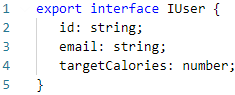
\includegraphics
	{../LaTeX/Images/npm_iuser.PNG}
	\caption{Interfața ”IUser”}
	\label{fig:55}
\end{figure}

\begin{figure}[!htb]
	\centering
	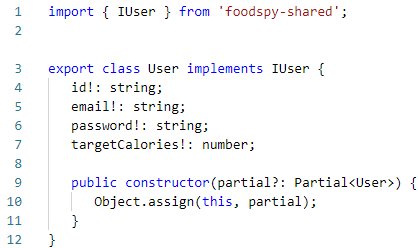
\includegraphics
	{../LaTeX/Images/npm_user.PNG}
	\caption{Implementarea interfeței ”IUser” în API}
	\label{fig:56}
\end{figure}


\section{Heroku}
Heroku este o platformă care pune la dispoziție posibilitatea de a construi, implementa și rula aplicații găzduite în cloud. Spre deosebire de Amazon Web Services sau Windows Azure, care oferă doar infrastructura în cloud necesară pentru a găzdui aplicația, Heroku oferă un serviciu de management asupra infrastructurii, care abstractizează toate detaliile legate de configurare și implementare. Astfel, Heroku permite dezvoltatorilor să concentreze toate resursele spre implementarea aplicației.
Heroku suportă o colecție de limbaje de programare și framework-uri, printre care JavaScript și Node.js.
\\ \\
Platforma pune la dispoziție toate uneltele necesare implementării unei aplicații, inclusiv administrarea mediului de rulare a aplicației și administrarea laturii DevOps. Din acest motiv, Heroku este un loc potrivit pentru a învăța despre microservicii și metodologii de implementare, precum livrarea continuă (”continuous delivery”). Mai mult decât atât, oferă un abonament destinat exclusiv studenților care permite utilizarea platformei pentru o perioadă de doi ani, suficient timp pentru a exersa orice limbaj de programare și orice șablon arhitectural.


\section{Docker}
Docker este o platformă cu sursă-deschisă folosită pentru construirea, implementarea, testarea și administrarea aplicațiilor bazate pe așa numitele containere. Containerele sunt pachete care conțin codul-sursă al aplicației și toate dependințele de care aplicația are nevoie pentru a funcționa corespunzător - biblioteci, unelte de sistem, cod-sursă și mediul de rulare (din engl. ”runtime environment”).\\
\begin{figure}[!htb]
	\centering
	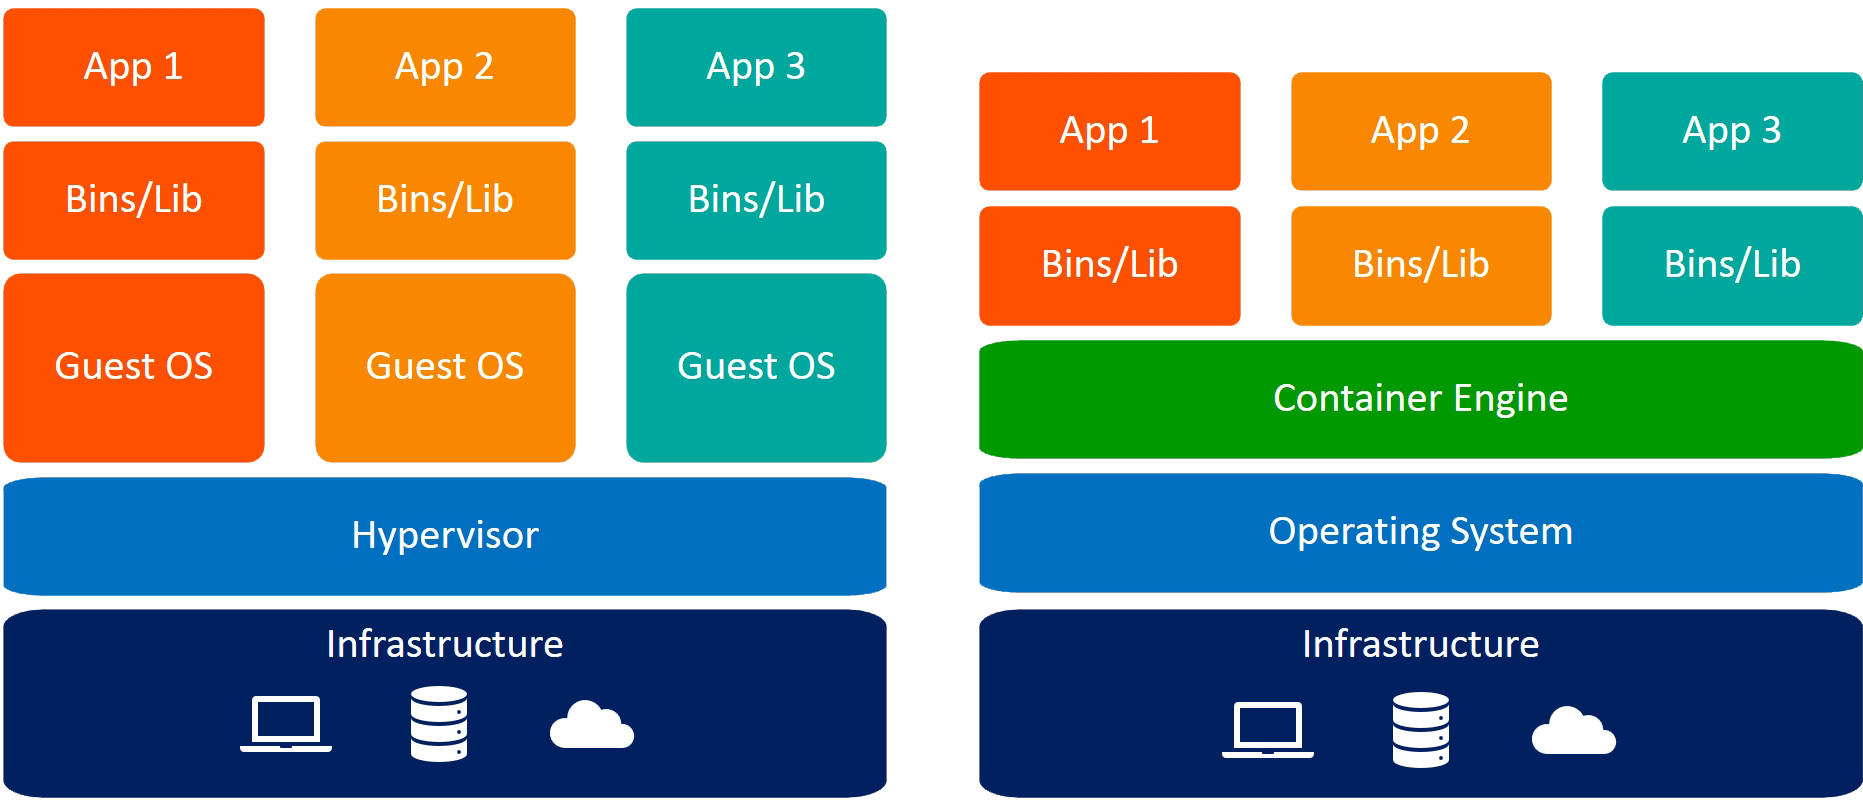
\includegraphics[width=1\textwidth]
	{../LaTeX/Images/docker.PNG}
	\caption{Mașină virtuală (stânga) vs. container(dreapta)}
	\label{fig:57}
\end{figure}

Câteva avantaje ale folosirii containerelor:
\begin{itemize}
	\item spre deosebire de o mașină virtuală, un container conține doar procesele sistemului de operare și dependințele necesare executării codului aplicației
	\item mult mai multe containere pot rula în paralel decât mașini virtuale, deoarece o mașină virtuală trebuie să suporte sarcina unui întregi instanțe de sistem de operare
	\item un container este mai ușor și mai rapid de implementat decât o mașină virtuală, astfel că sunt ideale în pipeline-uri ”continuous integration” și ”continuous delivery” (CI/CD)
\end{itemize}
Un ”DockerFile” este un fișier text care include instrucțiuni pentru creearea unei imagini Docker. Instrucțiunile sunt executate de ”Docker Engine”, iar rezultatul execuției reprezintă imaginea Docker.
O imagine Docker conține codul-sursă executabil al aplicației, dependințele acesteia și bibliotecile de care are nevoie pentru a rula sub formă de container. Când o imagine Docker este rulată, aceasta devine o instanță live, devine un container Docker. În timp ce o imagine Docker este un fișier ”read-only”, cu un container Docker se poate interacționa și manipula.


\section{Utilitare (Postman, Git și GitHub)}
Postman este un utilitar interactiv prin care se pot examina endpoint-urile unui API. Postman poate fi folosit pe tot parcursul dezvoltării unei aplicații deoarece dispune de o interfață grafică care permite construirea și trimiterea de request-uri HTTP. De asemenea, se poate folosi pentru citirea și validarea răspunsurilor oferite de către API. Un exemplu de request trimis direct din Postman către ”FoodSpyAPI”, care interoghează baza de date pentru alimente care au în componența numelui termenul ”magiun” este reprezentat în (Fig. \ref{fig:58}).

\begin{figure}[!htb]
	\centering
	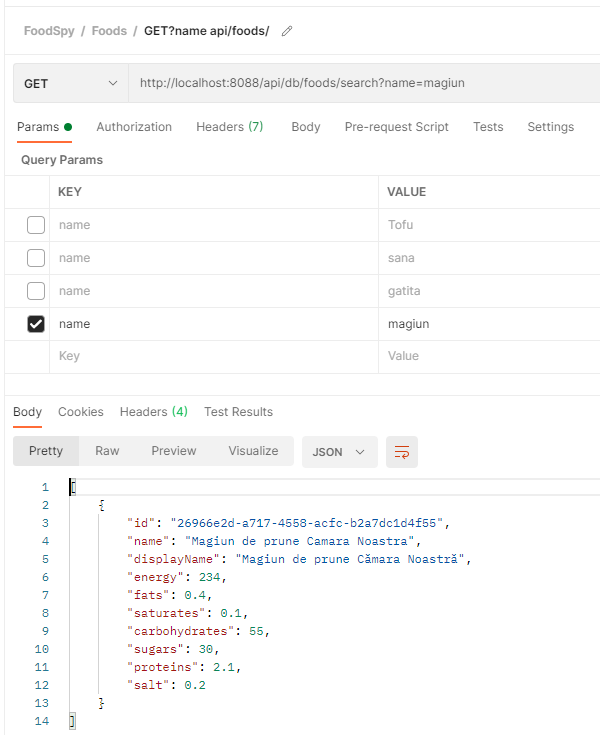
\includegraphics[width=1\textwidth]
	{../LaTeX/Images/postman_magiun.PNG}
	\caption{Request ”GET” trimis din Postman}
	\label{fig:58}
\end{figure}

%maybe add \\ \\ here
Git este un sistem de versionare distribuit care poate urmări schimbări în fișiere. Git este folosit de programatori pentru a colabora la scrierea codului-sursă în procesul de dezvoltare software. A fost creat în anul 2005 și a fost gândit pentru a fi eficient, pentru a păstra integritatea datelor și pentru a oferi suport pentru numeroase medii de dezvoltare.
\\ \\
Git urmărește schimbările în fișier pe toată durata dezvoltării software, ceea ce înseamnă că în orice moment, codul-sursă poate fi revizuit sau poate fi adus la o versiune precedentă.
\\ \\
Git se instalează și rulează pe sistemul local și nu are nevoie de conexiune la internet pentru a funcționa. Față de alte sisteme de versionare, Git este ușor de folosit și gratis și a fost gândit să lucreze în principal cu fișiere text, adică exact tipul de fișiere folosit pentru a salva cod-sursă. Întregul cod-sursă este menținut sub evidența sistemului de versionare într-un director care poartă numele de ”repository”. Avantajul major al Git este așa numitul ”branching model”. Prin procesul de ”branching” se pot crea ”ramuri”, care sunt copii independente ale repository-ului. Asta se traduce prin ușurința de a testa și implementa noi funcționalități în aplicație, fără a afecta munca celorlalți participanți la dezvoltarea aplicației.
\\ \\
GitHub este un serviciu de găzduire a unui repository. Este bazat exclusiv pe infrastructură cloud și este o bază de date care reține o colecție de repository-uri. GitHub este practic o versiune online a unui repository local și astfel oferă posibilitatea de a partaja un repository sau de a adăuga alți programatori care pot contribui în mod independent la dezvoltarea aplicației. Cu alte cuvinte, GitHub extinde funcționalitățile oferite de Git printr-o interfață intuitivă și unelte de management asupra unui repository. Un instantaneu al repository-ului care conține codul-sursă al aplicației ”FoodSpy” este reprezentat în (Fig. \ref{fig:59}). Se poate observa că branch-ul ”calculate-calories” a suferit 9 modificări de la momentul în care a fost clonat din branch-ul principal, adică ”master”.

\begin{figure}[!htb]
	\centering
	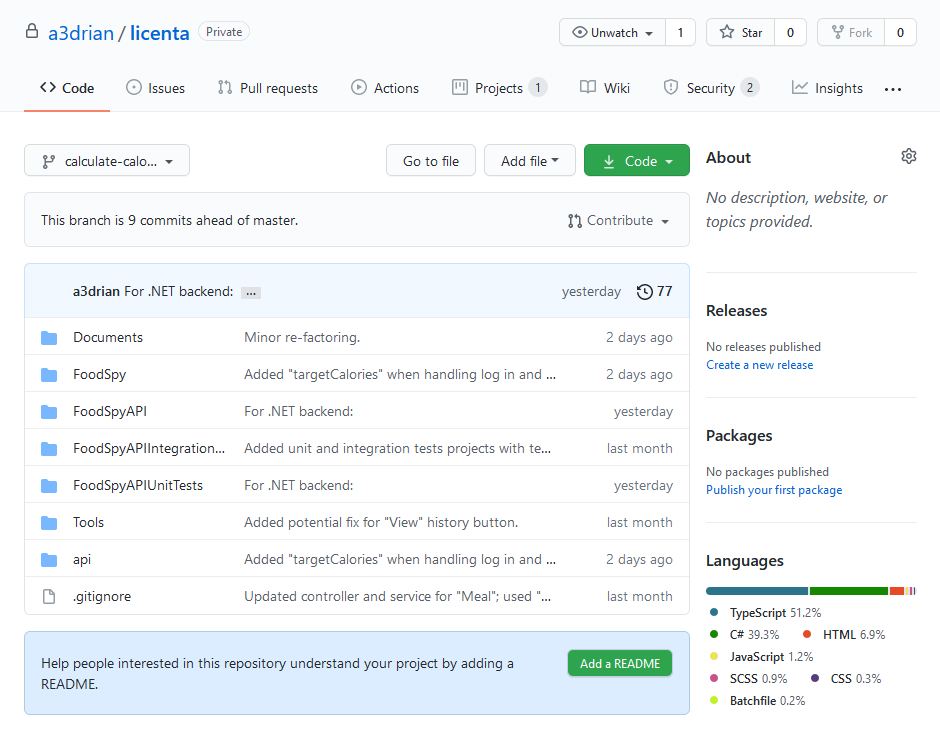
\includegraphics[width=1\textwidth]
	{../LaTeX/Images/github_repo.PNG}
	\caption{Repository-ul ”FoodSpy”}
	\label{fig:59}
\end{figure}